%
% Barren Planet - User Manual
% Main document source
%
% Copyright (C) Damian Gareth Walker 2022
% Manual Sections: Taking Your Turn
%
% Structure:
% The Player Turn screen
% - Windows
% - Map controls
% Selecting units and terrain
% - Friendly units
%   - Hits
%   - Power
%   - Range
%   - Armour
%   - Moves
% - Enemy units
% - Unoccupied terrain
% Moving units
% - Introductory
% - Move
% - Pathfinding
% - Performance
% - Blocked Paths
% Ending your turn
% The Turn Report
% Attacking units
% Stopping Play
%

% Chapter Heading
\chapter {Taking Your Turn}

% The Player Turn screen layout
\noindent
The top left of the {\it Player Turn} screen contains the battle map, just like in the {\it Mission Briefing} screen. The top right window is split in two. At the top there is a stats panel that shows information on units and terrain. At the bottom is a text window, currently mostly empty, onto which status messages will scroll. Currently it tells you there are no resources. Resources are not used in the first battle, so we can ignore that. We can also ignore the small pop-out in the middle of the screen that shows us our current resource level more prominently; that will stay at zero for the whole battle.

% The Player Turn screen image
\begin{figure}[h]
  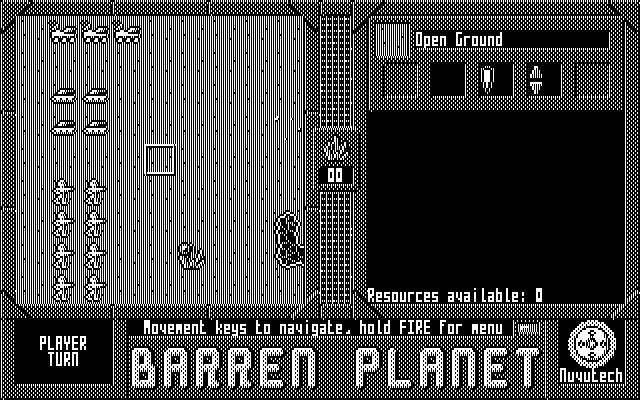
\includegraphics[width=\textwidth]{player-turn}
  \caption{The Player Turn screen}
\end{figure}

% Map controls
There is a difference between this map and the one on the {\it Briefing Screen}: this one has a square cursor, which should start in the middle of the map display. The movement keys allow you to move this cursor around the battlefield, highlighting particular units and terrain. Moving the cursor past the edge will scroll the display, if there is any more battlefield to show in that direction. As with other screens, holding {\it fire} brings up the menu in the bottom left.

% Getting Information
\section {Getting Information}

% Friendly units
\noindent
It's a good idea to start your turn by inspecting the individual units on the battlefield. The cursor is initially placed near your own units, so start with one of those. One of the humanoid figures, the Combat Droids, would be a good start. Move the cursor over to it and tap the {\it fire} button; this will call up the {\it Select} menu option which is the default option when pointing at one of your own units.

% The Unit Stats panel image
\begin{figure}[h]
  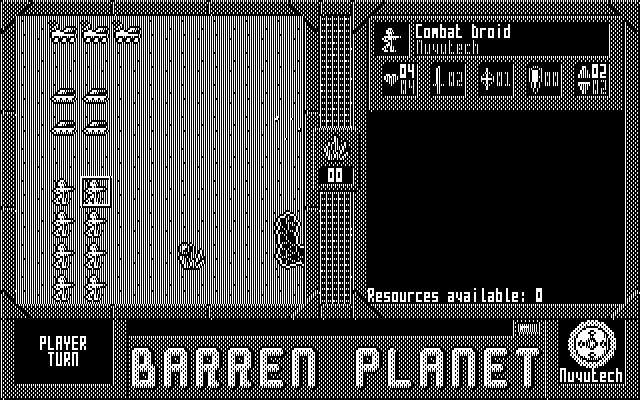
\includegraphics[width=\textwidth]{unit-stats}
  \caption{Stats for the Combat Droid shown at the top right.}
\end{figure}

% Unit statistics
The stats panel will change to illustrate the unit you just selected. You will see its icon in the panel, and its name, {\it Combat Droid}. The five square fields tell you of the unit statistics, which are these:
\begin{itemize}

  % Hit points
\item {\it Hit Points}, next to the heart symbol, show you the condition of your unit. The upper figure is the current number of hit points, which will be reduced when the unit is damaged in battle. The lower figure is the maximum number of hit points that the unit started out with.

  % Attack Power
\item {\it Attack Power}, next to the sword symbol, is the amount of damage that this unit can cause to an enemy unit in a single turn. When you attack an enemy, you will cause a random amount of damage between zero and this number, which will be deducted from the enemy's current hit points.

  % Attack Range
\item {\it Attack Range}, next to the target symbol, is the number of squares over which this unit can fire: 1 indicates it can only attack units in the next square, higher values indicate a longer range.

  % Armour
\item {\it Armour}, next to the shield symbol, is the number of points of damage that this unit can absorb from an enemy attack without affecting its hit points. When this unit is attacked, a random amount between 0 and this figure is deducted from the damage caused, before reducing the current hit point figure.

  % Movement
\item {\it Movement Points}, next to the arrow symbols, is the maximum number of squares over which a unit can move in a turn. The upper figure is the current number of movement points left, the lower figure is the number of movement points the unit will have at the start of every turn. Note that some terrain takes more than 1 movement point to traverse, and some terrain cannot be traversed at all by some units.
\end{itemize}

% Enemy Units
You can obtain similar information about enemy units. Move the cursor across the map to point at one of the enemy units, but be careful. The default menu option when pointing at an enemy unit is {\it Attack} and not {\it Select}, so you need to hold the {\it fire} control and move the menu cursor over to {\it Select} before releasing {\it fire}. The other difference between the friendly and enemy unit display is that you are not shown the current {\it Hit Points} or {\it Movement Points}, only the maximum for that type.

% Terrain
Information on terrain is also available. Select one of your own units again. Then move up to the ridge terrain at the top of the map. Hold {\it fire} and choose the {\it Select} option. Again you need to be careful, as {\it Select} is not the default option when pointing at empty terrain. The icon and name of the terrain will be shown in the stats panel. The three fields underneath tell you about the effect of that terrain on the currently selected unit.

% The Terrain Stats panel image
\begin{figure}[h]
  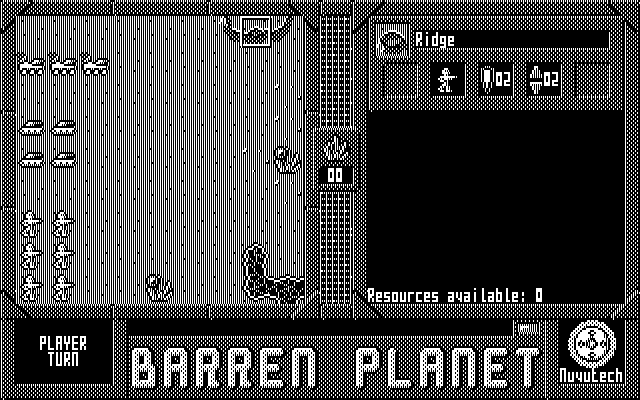
\includegraphics[width=\textwidth]{terrain-stats}
  \caption{Stats for Ridge terrain shown at the top right.}
\end{figure}
\begin{itemize}

  % Unit type
\item The first field contains the icon of your currently selected friendly unit, as a reminder of which unit type the other fields refer to.

  % Defence
\item The {\it Defence} figure, next to the shield symbol, shows how much the terrain protects that particular unit. This defence acts like extra armour; a number between 0 and this figure is deducted from the damage taken when this unit is attacked while sitting in this terrain. A dash means that the terrain doesn't protect this unit at all.

  % Movement
\item The {\it Movement Cost} figure, next to the arrow symbols, shows how many movement points it costs for the unit to move into this terrain. A dash means that the unit can't move into this terrain at all.

\end{itemize}

% New Unit types and the Terrain
When encountering a unit type on the battlefield for the first time, it is helpful to select it, and then get information on the various different types of terrain on the battlefield to get an idea of where that unit can most easily move and where it can dig in for maximum defence.

% Moving Units
\section{Moving Units}

% Introductory
\noindent
Now that you've examined the battlefield and the units in detail, it's time to get moving. You might have done this by accident already when examining terrain: that's all part of the learning process!

% Select
The first step to giving a unit its movement orders is to select it: move the cursor over to it and tap {\it fire} to select it. You'll see the stats panel indicate that this is your currently selected unit.

% Move
Then move the cursor to the empty spot where you want this unit to move. This will generally be in the direction of the enemy. You needn't stay within the range indicated by the unit's movement points, you can give orders to move towards a remote square even if your unit couldn't reach it this turn. Tap {\it fire} to select the {\it Move} option, which is the default when pointing at an empty square. The unit will move towards the destination.

% Pathfinding
Units will use intelligent {\it pathfinding} to work out the best route to their destination, moving around difficult or impassable terrain in the way. The computer will always find the most efficient path for your unit.

% Performance
On slower computers, this pathfinding might involve a noticeable delay before the unit begins to move. If you find this annoying, you can pick out the path yourself by moving to adjacent squares one at a time along your desired route. This may make the process more fluid when the unit is only moving one or two squares per turn.

% Blocked paths
Another problem occasionally arises when moving long distances: you may choose a destination that your unit cannot current find a path to, because there are units in the way. In this case you will have to either pick a square along the route that the unit can get to, or single-step your moves as just described.

% Moving the rest
Once you've moved the first unit, move the others towards the enemy. You may wish to use some of your units to occupy the crystal node squares as instructed in the mission briefing; Combat Droids are good units for holding these positions.

% Ending Your Turn
\section{Ending Your Turn}

% Introductory
\noindent
Once you have moved all the units, there is nothing more to do this turn. Your units will not yet be in firing range of the enemy, so combat will have to wait till future turns. So it's time to end your turn.

You do this by holding {\it fire} and selecting the {\it End Turn} option from the menu. The computer will then take its turn while you wait. Once the computer is done, you will be presented with the {\it Turn Report}.

% The Turn Report
\section{The Turn Report}

% Introductory
\noindent
While the computer was making its move, you will have seen a blank map window and a message asking you to wait. The computer's move is not shown to you in real time, so you will not know what the computer has been doing. This is what the {\it Turn Report} screen is for.

% The Terrain Stats panel image
\begin{figure}[h]
  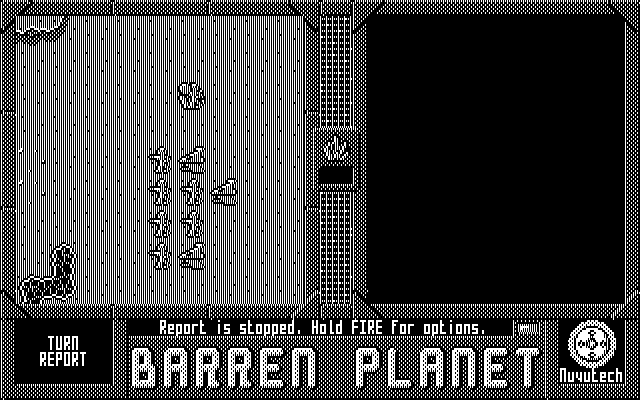
\includegraphics[width=\textwidth]{turn-report}
  \caption{The Turn Report screen shows what happens during the enemy's turn.}
\end{figure}

% The turn report
Every turn after an opponent has moved, assuming that the opponent did move, you begin with the {\it Turn Report} screen. Here you can see a replay of everything the opponent did: every move, every attack, and all the repairs and new unit construction that took place.

% Starting the report
Tap {\it fire} to select the default {\it Replay} option from the {\it Turn Report} menu. This will briskly go through all the computer's actions. The map window will show the units moving around, and the scrolling text window on the right will give information about interesting events like attacks, repair and new unit construction.

% Done with the report
Once the report is done, you can tap {\it fire} to select the default option {\it Proceed} to continue to the {\it Player Turn} screen to take your turn. Alternatively, if you want to see the report again, hold {\it fire} and select the {\it Replay} option which will show you all the computer's moves from the beginning of the turn.

% Attacking the Enemy
\section{Attacking the Enemy}

% Introductory
\noindent
After a number of turns, your units will come into firing range of the enemy. For most units in the first battle this means occupying the adjacent square, but Air Fighters can fire at units two squares away. Once within range, it is time to attack!

% Controls
Start by selecting one of your units that is ready to fire at the enemy, by moving the cursor over it and tapping {\it fire} to choose the default option {\it Select}. Then move the cursor to the enemy unit you want to attack, and tap {\it fire} again to choose {\it Attack}, which is the default option when pointing at an enemy.

% The Animation
Assuming the enemy really is in firing range, you will see a brief flash of fire from your unit and an explosion on the enemy. If this attack destroys the enemy, it will then disappear, otherwise it will remain on the battlefield but may have taken damage from your attack. A report in the text window will confirm the attack.

% An example of an attack
\begin{figure}[h]
  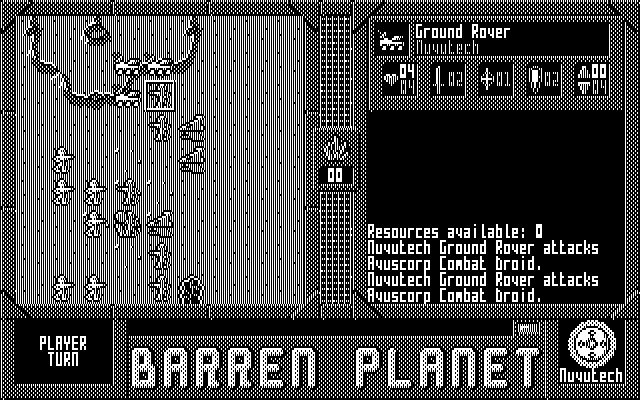
\includegraphics[width=\textwidth]{attack}
  \caption{A Ground Rover has just attacked a Combat Droid.}
\end{figure}

% Return Fire
If you are within the enemy unit's firing range, and if the enemy has movement points left, it may return fire, in which case you will see a flash of fire over the enemy and an explosion on your unit. If your unit is weak or the enemy is powerful, it is possible that your own unit could be destroyed in the attack. If this happens, your unit will disappear from the map and a report in the text window will confirm what happened.

% Expending Movement Points
When your unit attacks, the rest of its movement points are used up, so it can only fire once per turn. This also means that it will be unable to return fire if attacked during the enemy's next turn. If you want your unit to be able to return fire on the enemy you need to refrain from using it to attack this turn, and leave it with at least one movement point remaining at the end of your turn.

% Updated Status
Once the attack is done, the stats panel is updated to show the current status of your unit: its movement points will be zero, and its hit points may be reduced if the enemy returned fire and caused any damage.

% The rest of the game
Once all units have moved and attacked, you will want to end your turn as before. Continue attacking the enemy turn after turn, and also try to occupy the crystal nodes with your own units, and eventually, one way or another, the battle will come to an end.

% Stopping Play
\section{Stopping and Resuming Play}

% Exit Game
\noindent
A battle can take a long time to play through, and therefore a full campaign will take many times longer. It is very likely you will have to stop play at some point before the campaign is won. Almost every menu in the game has an {\it Exit Game} option at the bottom. Selecting this will save the current game and drop back to DOS. When you next run {\bf \it Barren Planet}, you will return to the point where you left off.

% New Game
At some point, you might want to leave off one game and start another. Along with the {\it Exit Game} option, most menus have a {\it New Game} option too. This will save the current game, so that you can return to it later, and take you to the {\it New Game} screen.

% Multiple Games
You can have multiple games in progress at once. To resume a previously saved game at the {\it New Game} screen, move the highlight bar up to {\it Game:} and use the $\leftarrow$ and $\rightarrow$ controls to cycle through the saved games. Each is identified by the date and time the game was started. Cycling $\leftarrow$ all the way will bring you back to {\it New Game}. Note that when you have a saved game selected, you cannot change the other options ({\it Campaign}, {\it Nuvutech} and {\it Avuscorp}) for that game. Once the game has started, these are fixed.
